\documentclass[10pt,twocolumn,letterpaper]{article}

\usepackage{cvpr}
\usepackage{times}
\usepackage{epsfig}
\usepackage{graphicx}
\usepackage{amsmath}
\usepackage{amssymb}

\usepackage{url}

% Include other packages here, before hyperref.
\usepackage{algorithm}
\usepackage{algpseudocode}
\usepackage{xcolor}

% If you comment hyperref and then uncomment it, you should delete
% egpaper.aux before re-running latex.  (Or just hit 'q' on the first latex
% run, let it finish, and you should be clear).
%\usepackage[pagebackref=true,breaklinks=true,letterpaper=true,colorlinks,bookmarks=false]{hyperref}

\cvprfinalcopy % *** Uncomment this line for the final submission

\def\cvprPaperID{****} % *** Enter the CVPR Paper ID here
\def\httilde{\mbox{\tt\raisebox{-.5ex}{\symbol{126}}}}

% Pages are numbered in submission mode, and unnumbered in camera-ready
\ifcvprfinal\pagestyle{empty}\fi
\begin{document}

%%%%%%%%% TITLE
\title{K-Means Clustering: comparison between a sequential and parallel implementation}

\author{Beatrice Paoli\\
{\tt\small beatrice.paoli@stud.unifi.it}
}

\maketitle
\thispagestyle{empty}

%%%%%%%%% ABSTRACT
\begin{abstract}
	The goal of this paper is to present two implementations of the k-means clustering algorithm: a sequential version and a parallel one. Both are written in C++, with the parallel version obtained with the use of OpenMP. This paper also provides a performance analysis and comparison between the two versions in terms of execution times and speedup and how this values change with different inputs (dataset size and number of centers) and different numbers of threads. 
\end{abstract}

%-------------------------------------------------------------------------

\section{The Algorithm}

The K-means algorithm is a parametrized clustering technique that allows to partition a dataset of points or observations into K clusters. Points in the same cluster minimize the distance from the center of the cluster (called \textit{prototype}). 

Many metrics of distances can be used depending on the dataset to cluster, for this implementation the dataset is comprised of 2D points and distances are measured with the Euclidean distance.

The algorithm is composed by few steps, with two main phases alternated between each other: the \textit{Assignment} phase and the \textit{Update} phase. %\ref{alg:KMeansAlg}

\begin{algorithm}
	\label{alg:KMeansAlg}
	\caption{K-Means Clustering}
	\begin{algorithmic}
		\Require K = number of clusters to create
		\vspace{0.5cm}
		
		\State Select K points as initial centroids of the clusters
		\While{Centroids keep changing}
		\For{each point $p$}
		\State Assign $p$ to the cluster with the closest centroid
		\EndFor
		\For{each cluster $c$}
		\State Update the centroid of $c$
		\EndFor
		\EndWhile
		\State \Return clusters
		
	\end{algorithmic}
\end{algorithm}

The algorithm converges after few steps to a local minimum, depending on the choice of the initial centroids. In the implementation presented in this paper, the starting centroids are chosen randomly from the dataset in input. Therefor, different runs of the algorithm on the same dataset and the same number of centroids can yield different results. Other initialization methods can be used to obtain the gloabl optimum more consistently.

%-------------------------------------------------------------------------

\section{Implementation}
The details of the implementations of the function \textit{kMeansClustering()} are presented in the following paragraphs.

\subsection{Classes}
\begin{itemize}
	\item \textbf{Point}: this class is used to represent the points of the input dataset to cluster. It has three members: \textit{x} and \textit{y} for the coordinates, and \textit{clusterId} for the id of the cluster to which the point has been assigned. 
	
	The class also has two constructors and the method \textit{dist()} to compute the Euclidean distance between two points.
	
	\item \textbf{Cluster}: this class is used to represent the clusters created by the algorithm. Each cluster has an \textit{id} ranging from 0 to $K - 1$, a \textit{Point} for the current mean or centroid of the cluster, two fields to compute the partial sums of all points for each coordinate, \textit{tempSumX} and \textit{tempSumY}, and an integer for the size of the cluster.
	
	Aside from the constructor, the class has two main methods:
	\begin{itemize}
		\item \textit{addPoint()}: is used during the Assignment phase; it adds a point to the cluster by increasing the \textit{size} counter and by adding its coordinates to the partial sums.
		\item \textit{updateCentroid()}: is used during the Update phase; it computes the new mean of the cluster by using the sums of the coordinates computed before and the size of the cluster. After the update, \textit{tempSumX}, \textit{tempSumY} and \textit{size} are resetted to 0, ready for a new iteration of the algorithm.
	\end{itemize}
\end{itemize}

\subsection{kMeansClustering}
The function \textit{kMeansClustering()} accepts three parameters: an integer \textit{k} for the number of clusters to output, a \textit{std::vector} of type \textit{Point} for the dataset, and an integer for the number of iterations of the algorithm to perform. The last parameter is optional and has a default value of 20.

The function starts by performing a random initialization of the clusters by choosing $k$ points as initial centroids.

In a \textit{for} cycle bounded by the number of iterations to perform, the function alternates the assignment and update steps.
In the assignment step, for each point we find the cluster with the closest centroid and then update the point's \textit{clusterId} and call the cluster's method \textit{addPoint()} to update the partial sums of the future centroid.

The update step is limited to a simple \textit{for} cycle over the clusters to call \textit{updateCetroid()} to update all the centroids with the current points assignment. 

\subsection{OpenMP Parallelization}
To achieve parallelization it was necessary to use only a few parallel directives.

The assignment step is embarrassingly parallel since the search and assignment of each point to a cluster is independent from one another.
So a \verb"#pragma omp parallel for" statement was used on the points loop to use threads to parallelize the computation.

\begin{algorithm}
	\label{alg:KMeansAlgParallel}
	\caption{Parallel K-Means Clustering}
	\begin{algorithmic}
		\Require K = number of clusters to create
		\vspace{0.5cm}
		
		\State Select K points as initial centroids of the clusters
		\While{Centroids keep changing}
		\State \textcolor{orange}{\#pragma omp parallel for}
		\For{each point $p$}
		\State Assign $p$ to the cluster with the closest centroid
		\EndFor
		\For{each cluster $c$}
		\State Update the centroid of $c$
		\EndFor
		\EndWhile
		\State \Return clusters
		
	\end{algorithmic}
\end{algorithm}

Since the workload for each thread is similar the default static scheduler is used.

However, each thread accesses the shared clusters to call \textit{addPoint()} and update the internal cluster variable. Without any synchronization mechanism, this introduces a race condition on the algorithm that leads to incorrect results.

The method \textit{addPoint()} only performs three sums over the variables \textit{tempSumX}, \textit{tempSumY} and \textit{size}, so three \verb"#pragma omp atomic" were used to ensure the correct update of the variables and avoid the race condition.

The update step, as stated before, is limited to a simple \textit{for} loop over the clusters to update each centroid by performing only two divisions. This step is also embarrassingly parallel but the computations performed inside the loop are far too simple and the number of clusters is much smaller compared to the number of points. For these reasons it would be counter-productive to paralleliza this step, as the overhead of thread management would decrease the performance of the algorithm.

\section{Performance Analysis}
In order to compare the performance of a sequential algorithm with its parallel version we can use the concept of \textit{speedup}.

Speedup is measured as the ratio between the execution time of the sequential algorithm and the parallel one.

\[S = \frac{t_s}{t_p}\]

Ideally, we should look for \textit{perfect speedup} or even \textit{linear speedup}, meaning $S$ should be equal or similar to the number of processors used to perform the parallel algorithm.

The experiments were performed on a Intel Core i7-1165G7 with 8 logical cores, with 2D input datasets generated with \textit{scikit-learn} in Python.

Since the algorithm has the hyperparameter $K$ for the number of clusters, different experiments were performed with varying $K$ and fixed $N$ (number of points), and viceversa.

\begin{figure}[H]
	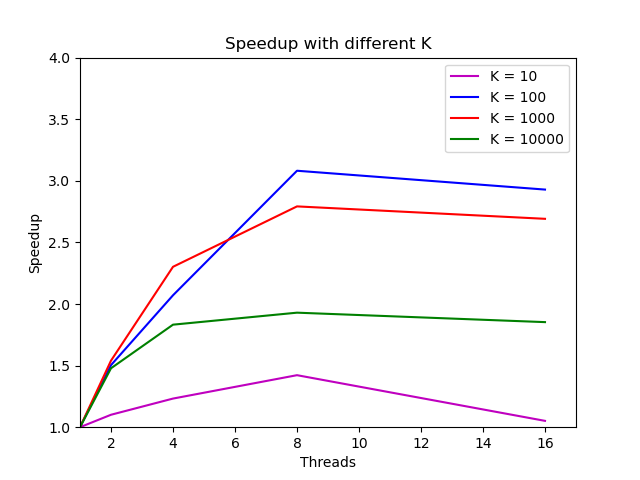
\includegraphics[width=\linewidth]{images/speedup_by_k.png}
	\caption{Speedup K Means Clustering con N = 100000.}
	\label{fig:speedup_k}
\end{figure}

In Figure \ref{fig:speedup_k} we have the different speedups for different numbers of threads used and different values of $K$. We can see how the speedup increases up to 8 threads as expected, but in a sub-linear way.
The results also depend on the value of $K$ chosen. 

For small $K$, the speedup are significantly worse and deteriorate almost to 1 for a high number of threads. Since the work of each thread consists mainly on computing all the distances between a point and all centroids to find the closest cluster, so for small numbers of $K$ the computation of each thread can become too little and the gain in speedup is lost due to thread management.


\begin{table}
\begin{center}
\begin{tabular}{|c|c|c|}
\hline
Threads & Execution Time & Speedup \\
\hline
1 & 12.106 & 1 \\ 
2 & 7.860 & 1.540 \\
4 & 5.259 & 2.302 \\
8 & 4.335 & 2.792 \\ 
16 & 4.498 & 2.691 \\
\hline
\end{tabular}
\end{center}
\caption{Execution Times for K = 1000 and N = 100000.}
\label{tab:speedup_k_n}
\end{table}

\begin{figure}[H]
	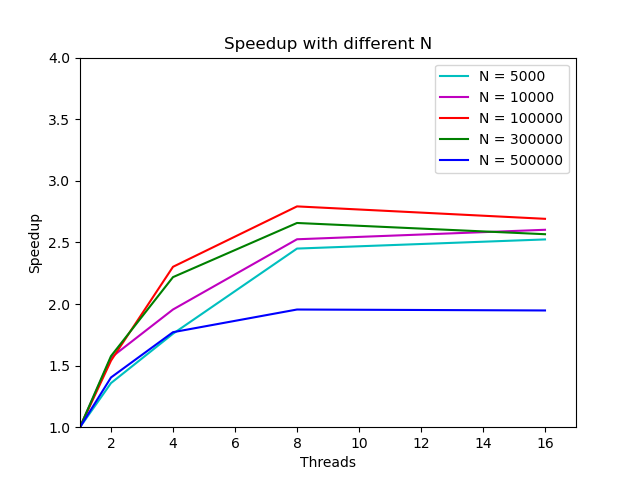
\includegraphics[width=\linewidth]{images/speedup_by_n.png}
	\caption{Speedup K Means Clustering con K = 1000.}
	\label{fig:speedup_n}
\end{figure}

In Figure \ref{fig:speedup_n} we have the speedup trends for different sizes $N$ of datasets. As before, the values increase up to 8 in a sub-linear way.


\end{document}
